\documentclass[journal]{IEEEtran}
%\IEEEoverridecommandlockouts
% The preceding line is only needed to identify funding in the first footnote. If that is unneeded, please comment it out.

% listings package for code blocks
\usepackage{listings}
\usepackage{xcolor}
\usepackage{cite}
\usepackage{verbatim}
\usepackage{graphicx}
\usepackage{parskip}

\begin{document}

% overfull \hbox .. too wide 
\setlength{\emergencystretch}{12pt}
%\setlength{\parskip}{0pt} % 1ex plus 0.5ex minus 0.2ex}
\setlength{\parindent}{10pt}

\definecolor{codegreen}{rgb}{0,0.6,0}
\definecolor{codegray}{rgb}{0.5,0.5,0.5}
\definecolor{codepurple}{rgb}{0.58,0,0.82}
\definecolor{backcolour}{rgb}{0.95,0.95,0.92}

\lstdefinestyle{mystyle}{
    backgroundcolor=\color{backcolour},   
    commentstyle=\color{codegreen},
    keywordstyle=\color{magenta},
    numberstyle=\tiny\color{codegray},
    stringstyle=\color{codepurple},
    basicstyle=\ttfamily,
    breakatwhitespace=false,         
    breaklines=true,      
    postbreak=\mbox{\textcolor{red}{$\hookrightarrow$}\space},           
    captionpos=b,
}

\lstset{style=mystyle}

\title{Evaluating Classifications Models using Confusion Matrices}

\author{
\IEEEauthorblockN{Lillian Mueller}
\IEEEauthorblockA{lmuelle1@umd.edu}
}

\maketitle

\begin{abstract}
\label{log:abstract}
\end{abstract}

\section{Introduction}

Predicting the classification of Iris flowers has been proven possible time and time again. In previous cases, this classification has been modeled using decision trees, logistic regression, and K-nearest neighbor classification models \cite{b1}-\cite{b3}. Using the same iris dataset as previous studies, evaluating which model may provide the greatest profit is key to determining whether a model is effective for business applications. To determine which model maximizes profit, confusion matrices will be used to quantify the cost of inaccurate classifications versus the benefit of accurate classifications. As a reminder, the iris dataset consists of 150 data entries, each containing the petal length, petal width, sepal length, sepal width, and class of iris plant. Each model aims to predict the class of the iris plant based on the given features. 

Confusion matrices display outcomes from a model and sort those outcomes by predicted and actual values \cite{b4}. An analyst can then visually see how many outcomes from the model were classified correctly, which are referred to as true positives (TP) and true negatives (TN). The analyst can also see how many outcomes were classified incorrectly as well as which classification the point was confused with; these are referred to as false positives (FP) and false negatives (FN). Using this matrix, expected rates of the correct classifications versus the incorrect classifications can be found to calculate the overall expected value of the model \cite{b5}. Replicating the methodology to find each expected value for the models will aid in determining which model is most effective at maximizing profit. 

The methodology followed to determine the most cost effective model is described in Section ~\ref{sec:methodology}. Results are discussed in Section ~\ref{sec:results}. And finally lasting comments and future research can be found in Section ~\ref{sec:discussion}.


\section{Methodology}
\label{sec:methodology}

This investigation entails using various classes from the library \lstinline{scikitlearn}. To develop the models: the \lstinline{DecisionTreeClassifier} class from the \lstinline{tree} module, the \lstinline{LogisticRegression} class from the \lstinline{linear_model} module, and the \lstinline{KNeighbors} function from the \lstinline{neighbors} module. Each was used to develop the decision tree model, the logistic regression model, and the k-nearest neighbors model respectively. To develop the confusion matrices and accuracy/precision scores of each model ,  \lstinline{sklearn}'s \lstinline{metrics} module was used. Other Python libraries were used along the was as well to help handle the data which includes \lstinline{matplotlib.pyplot}, \lstinline{pandas}, and \lstinline{numpy}. 

First, the Iris dataset was loaded as an \lstinline{sklearn.utils.Bunch} object called \lstinline{iris_data} via the \lstinline{load_iris()} function. This object is similar to a Python dictionary. To make the data easier to read, it was transformed into the \lstinline{df_iris} dataframe, where the data parameter was set as the \lstinline{data} attribute of the dataset and the columns parameter as the \lstinline{feature_names} attribute. A new column called “class” was added to this dataframe which contains the \lstinline{target} variable of the Iris dataset; this is the class of the Iris plant - setosa, versicolor, or virginica. Since the \lstinline{target} attribute contains an array with values from 0-2, the \lstinline{replace} function was used to map these numerical values to their corresponding classifications: setosa for \(0\), versicolor for \(1\), and virginica for \(2\). 

After the Iris dataset was loaded in and processed, it was split into a train group and test group using the \lstinline{test_train_split} function, with 2/3 of the data as the train group and the remainder as the test group. 

Next, the models were developed. For each model, similar methods were used as describe in previous studies \cite{b1}-\cite{b3}. For context, the decision tree model was developed with the Gini impurity criterion, the logistic regression model was developed without any penalty, and the KNN model was developed using k=10 and the Euclidean distance metric. These were determined to be the most effective version of each model in their respective investigation. Additionally, all models were trained using the same training subset of the dataset.

After creating these models, they were applied to the testing subset of the dataset. The  classification predictions were then compared to the actual testing data classifications. A confusion matrix was created for each model using the \lstinline{confusion_matrix()} method from the \lstinline{metrics} module. Using the \lstinline{ConfusionMatrixDisplay} method, also from \lstinline{metrics}, a depiction of the matrix was developed. To generate further evaluation measures, the models' accuracy, precision, and recall scores were calculated using \lstinline{accuracy_score()}, \lstinline{precision_score()}, and \lstinline{recall_score()} respectively, all methods from the \lstinline{metrics} module. These values can also be calculated using the \lstinline{classification_report} method which also calculates the f-score (measure of accuracy using the recall and precision) and weighted and macro average accuracies. 

Once the confusion matrix and general metrics were calculated for each model, the expected value for each model could be calculated. The expected value is calculated by summing the products of each error rate multiplied by the corresponding cost or benefit. Error rates are calculated by dividing the outcomes counts from the confusion matrix by the number of total outcomes. The confusion matrix consists of counts of true positives, true negatives, false positives, and false negatives. The following diagram depicts this process. 

\begin{figure}[h!]
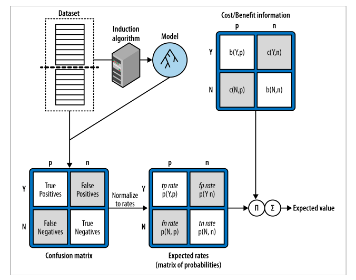
\includegraphics[scale=1]{expectedValDiagram.png}
\centering
\caption{Expected Value Calculation Diagram}
\label{fig:expectedValDiagram}
\end{figure}

For this case, since there are 3 classifications, setosa, virginica, and versicolor, the diagrams will correspond to table \ref{table:cm-meaning}.

\begin{table}[h!]
\centering
\begin{tabular}{ c || c | c | c }
& 0 = setosa &  1 = versicolor &  2 = virginica \\
\hline
\hline
0 & predicted : 0 & predicted : 1 & predicted : 2 \\
& actual : 0 & actual : 0 & actual : 0 \\
\hline
1 & predicted : 0 & predicted : 1 & predicted : 2 \\
& actual : 1 & actual : 1 & actual : 1 \\
\hline
2 & predicted : 0 & predicted : 1 & predicted : 2 \\
& actual : 2 & actual : 2 & actual : 2 \\
\end{tabular}
\caption{Confusion Table Meaning for Iris Dataset}
\label{table:cm-meaning}
\end{table}

To start this calculation, the cost/benefit information was developed. For correct classifications, I assigned a benefit of 1 and for each incorrect classification, I assigned a cost of -1. The final cost/benefit matrix is shown in Table \ref{table:costmatrix}.

\begin{table}[h!]
\centering
\begin{tabular}{ c || c | c | c }
& Predicted: 0 = setosa &  1 = versicolor &  2 = virginica \\
\hline
\hline
Actual: 0 & 1 & -1 & -1 \\
1 & -1 & 1 & -1 \\
2 & -1 & -1 & 1 \\
\end{tabular}
\caption{Cost/benefit Information}
\label{table:costmatrix}
\end{table}

In order to find the expected rates of each outcome, each value in the confusion matrix was divided by the sum of the confusion matrix. Each rate is then multiplied by the corresponding value in the cost/benefit matrix. Finally, to find the expected profit for the model, all values are summed. 

\section{Results}
\label{sec:results}

\subsection{Confusion Matrices}

After the development of each model, a confusion matrix was created to better understand the performance of the model on the testing dataset. Figures \ref{fig:cm-dtree}, \ref{fig:cm-logreg}, and \ref{fig:cm-knn} show the matrices for the decision tree model, the logistic regression model, and the KNN model respectively. 

\begin{figure}[h!]
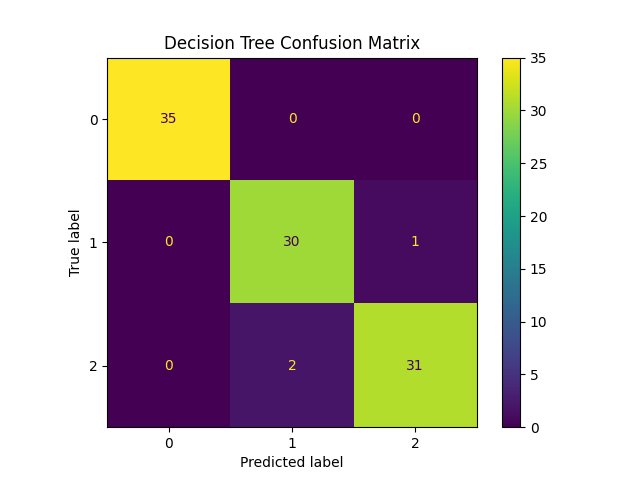
\includegraphics[scale=.5]{dtree_cm.png}
\centering
\caption{Confusion Matrix for Decision Tree Model}
\label{fig:cm-dtree}
\end{figure}

\begin{figure}[h!]
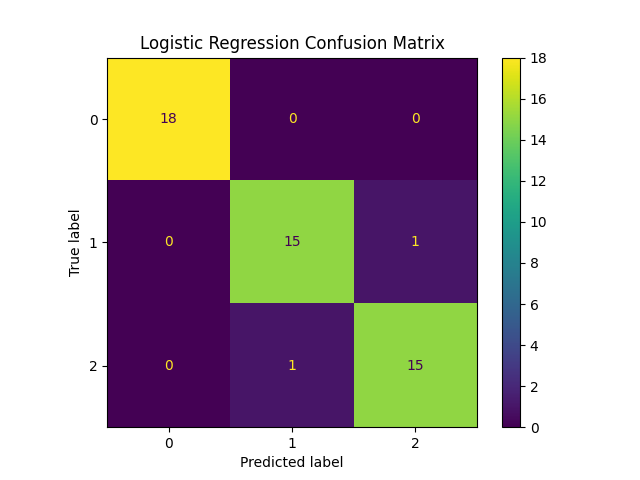
\includegraphics[scale=.5]{logR_cm.png}
\centering
\caption{Confusion Matrix for Logistic Regression Model}
\label{fig:cm-logreg}
\end{figure}

\begin{figure}[h!]
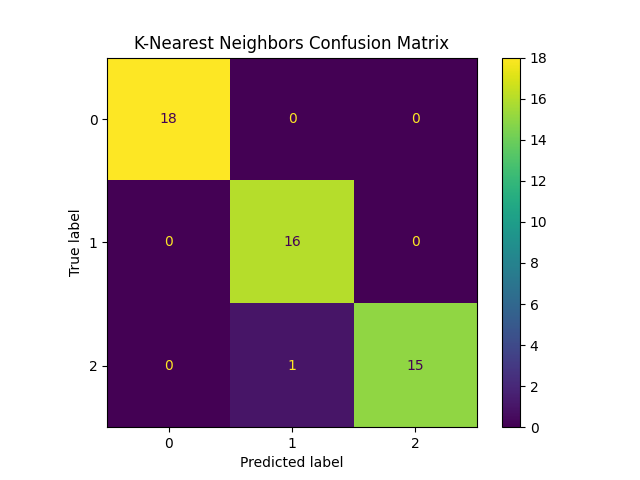
\includegraphics[scale=.5]{knn_cm.png}
\centering
\caption{Confusion Matrix for K-Nearest Neighbor Model}
\label{fig:cm-knn}
\end{figure}

Looking at the matrices, all the models are fairly accurate at classifying each iris flower. Each model was tested with 50 data entries, since the data was trained on 2/3 of the total dataset. The numbers in each square represent the number of outcomes for each event. These events correspond to \ref{table:cm-meaning}. From these matrices alone, an analyst may conclude that the KNN model has the best performance as its associated confusion matrix shows the least amount of misclassified events. 

\subsection{Evaluating Expected Profit}

After following the procedures in Section~\ref{sec:methodology}, the following expected profits were found. 

\begin{table}[h!]
\centering
\begin{tabular}{ c | c }
Model & Expected Profit \\
\hline
Decision Tree & 0.84 \\
Logistic Regression & 0.92 \\
KNN & 0.96
\end{tabular}
\caption{Expected Values}
\label{table:exVals}
\end{table}

An analyst can conclude that the K-Nearest Neighbor model will yield the most profit and therefore maximize profit. This makes sense as flowers, and organisms in general, are classified by similarities and KNN models model similarity. 

These results also reinforce past investigations. When using cross validation to compare the decision tree, logistic regression, and KNN models, the KNN model was also found to be the most stable for the iris dataset \cite{b3}. 

\section{Discussion}
\label{sec:discussion}


\begin{thebibliography}{00}
\bibitem{b1} L. Mueller and R. Hong, “Investigating Decision Trees”.
\bibitem{b2} L. Mueller and R. Hong, “Iris Classification Using Logistic Regression”.
\bibitem{b3} L. Mueller and R. Hong, “Evaluating the Performance of K-Nearest Neighbors Classification”.
\bibitem{b4} “Confusion Matrix - an overview | ScienceDirect Topics.” Accessed: Oct. 26, 2023. [Online]. Available: https://www.sciencedirect.com/topics/engineering/confusion-matrix
\bibitem{b5} F. Provost and T. Fawcett, Data Science for Business: What You Need to Know About Data Mining and Data Analytic Thinking, First edition (2005).

\end{thebibliography}

\end{document}